\subsection{Experimental Results on TR-MF} \label{subsec:exp_basic}%from Chung-Yi
We compare our TR-MF with conventional MF (i.e. MF without temporal regularization), Linear Interpolation~(LI), Applying K-nearest neighbour Estimation~(AKE), Data Estimation using Statistical Model~(DESM), Spatial temporal imputation~(STI) and Multiple Inputation (MI).
%We implemented AKE, DESM, STI, and for MI we use the EM-imputation from LISREL.  
Note that we only know the location information of 8 out of 20 sensors in traffic data set, but the pairwise distance values are mandatary to execute DESM and STI. For them, we simply assume the distances are all equal.

%validation setting
%Table \ref{table:berkeley_random_hum}, \ref{table:berkeley_random_light} and \ref{table:berkeley_random_tem} show the results of different models random split on Berkeley data set. In the plot, the x-axis represents the missing ratio. Conceivably the difficulty of an imputation task arises with th increase of missing ratio, therefore we can see that the slopes for most of the lines in the plot are nonpositive. Also note that to highlight the difference between the better models, we cut the overflowed RMSE values of the inferior models to the maximum values that can be displayed in the plot. That says, the flat lines on top of the plots usually indicate the exact RMSE is even higher than what has been shown.

Figure \ref{fig:berkeley_random_hum}, \ref{fig:berkeley_random_light}, \ref{fig:berkeley_random_tem}, \ref{fig:traffic_random_hum} and \ref{fig:traffic_random_tem} show the result of random missing. The outcome indicates several interesting facts. First, TR-MF outperforms the original MF significantly, which demonstrates the effectiveness of the temporal regularization. In general, TR-MF shows significant improvement over all the other methods. On the other hand, LT is quite competitive on berkeley data, especially for lower missing ratio cases. This is because the sampling rate of Berkeley data set is fairly high, so using only temporal correlation is sufficient to obtain decent results. In a data with lower sampling rate as the traffic data, the spatial-oriented methods such as AKE outperforms LI. 

%\begin{table}[htbp]
%\setlength{\tabcolsep}{2pt}
%\centering
%\caption{RMSE of (Berkeley, random, humidity)}
%\label{table:berkeley_random_hum}
%\begin{tabular}{ r | r r r r r r}
%	train	&LI	&TR-MF	&AKE	&DESM	&STI &MI\\ \hline
%	10\% & $ 0.171_{(2)} $ & $ \mathbf{ 0.142_{(1)} } $ & $ 0.264_{(3)} $ & $ 0.544_{(4)} $ & $ 1.220_{(5)} $&$0.190$ \\
%	20\% & $ 0.127_{(2)} $ & $ \mathbf{ 0.114_{(1)} } $ & $ 0.244_{(3)} $ & $ 0.318_{(4)} $ & $ 1.472_{(5)} $ &$ 0.151$\\
%	40\% & $ 0.095_{(2)} $ & $ \mathbf{ 0.092_{(1)} } $ & $ 0.199_{(3)} $ & $ 0.219_{(4)} $ & $ 1.648_{(5)} $ &$ 0.101$\\
%	60\% & $ 0.085_{(2)} $ & $ \mathbf{ 0.082_{(1)} } $ & $ 0.181_{(4)} $ & $ 0.180_{(3)} $ & $ 1.649_{(5)} $ &$ 0.092$\\
%	80\% & $ \mathbf{ 0.075_{(1)} } $ & $ 0.076_{(2)} $ & $ 0.127_{(3)} $ & $ 0.160_{(4)} $ & $ 1.604_{(5)} $ &$0.079$ \\
%	85\% & $ \mathbf{ 0.074_{(1)} } $ & $ 0.075_{(2)} $ & $ 0.121_{(3)} $ & $ 0.148_{(4)} $ & $ 1.549_{(5)} $ &$0.082$ \\ \hline
%	rank &1.67 &1.33 &3.17 &3.83 &5.00 \\
%\end{tabular}
%\end{table}
%
%\begin{table} [htbp]
%\setlength{\tabcolsep}{2pt}
%\centering
%\caption{RMSE of (Berkeley, random, light)}
%\label{table:berkeley_random_light}
%\begin{tabular}{ r |  r r r r r r}
%	train	&LI	&TR-MF	&AKE	&DESM	&STI &MI\\ \hline
%	10\% & $ 52.9_{(2)} $ & $ \mathbf{ 35.5_{(1)} } $ & $ 61.2_{(3)} $ & $ 6250.4_{(5)} $ & $ 258.2_{(4)} $ &$103.3$ \\
%	20\% & $ 38.7_{(2)} $ & $ \mathbf{ 28.2_{(1)} } $ & $ 53.0_{(3)} $ & $ 215.9_{(4)} $ & $ 311.0_{(5)} $ &$70.3$\\
%	40\% & $ 29.9_{(2)} $ & $ \mathbf{ 21.2_{(1)} } $ & $ 41.4_{(3)} $ & $ 356.7_{(5)} $ & $ 356.3_{(4)} $ &$48.2$\\
%	60\% & $ 25.0_{(2)} $ & $ \mathbf{ 17.2_{(1)} } $ & $ 33.7_{(3)} $ & $ 112.6_{(4)} $ & $ 366.9_{(5)} $ &$39.9$\\
%	80\% & $ 23.9_{(2)} $ & $ \mathbf{ 17.7_{(1)} } $ & $ 27.9_{(3)} $ & $ 41.7_{(4)} $ & $ 363.3_{(5)} $ &$42.1$\\
%	85\% & $ 20.9_{(2)} $ & $ \mathbf{ 14.4_{(1)} } $ & $ 24.3_{(3)} $ & $ 44.4_{(4)} $ & $ 354.2_{(5)} $ &$29.3$\\ \hline
%	rank &2.00 &1.00 &3.00 &4.33 &4.67 \\
%\end{tabular}
%\end{table}
%
%\begin{table}[htbp]
%\setlength{\tabcolsep}{2pt}
%\centering
%\caption{RMSE of (Berkeley, random, temperature)}
%\label{table:berkeley_random_tem}
%\begin{tabular}{ r | r r r r r r}
%	train	&LI	&TR-MF	&AKE	&DESM	&STI &MI\\ \hline
%	10\% & $ 0.070_{(2)} $ & $ \mathbf{ 0.046_{(1)} } $ & $ 0.112_{(3)} $ & $ 0.298_{(4)} $ & $ 0.506_{(5)} $ &$0.121$\\
%	20\% & $ 0.042_{(2)} $ & $ \mathbf{ 0.032_{(1)} } $ & $ 0.111_{(3)} $ & $ 0.167_{(4)} $ & $ 0.584_{(5)} $ &$0.098$\\
%	40\% & $ 0.027_{(2)} $ & $ \mathbf{ 0.023_{(1)} } $ & $ 0.080_{(3)} $ & $ 0.095_{(4)} $ & $ 0.644_{(5)} $ &$0.094$\\
%	60\% & $ 0.021_{(2)} $ & $ \mathbf{ 0.018_{(1)} } $ & $ 0.053_{(3)} $ & $ 0.067_{(4)} $ & $ 0.637_{(5)} $ &$0.091$\\
%	80\% & $ 0.016_{(2)} $ & $ \mathbf{ 0.015_{(1)} } $ & $ 0.043_{(3)} $ & $ 0.048_{(4)} $ & $ 0.611_{(5)} $ &$0.078$\\
%	85\% & $ 0.019_{(2)} $ & $ \mathbf{ 0.016_{(1)} } $ & $ 0.034_{(3)} $ & $ 0.048_{(4)} $ & $ 0.593_{(5)} $ &$0.082$\\ \hline
%	rank &2.00 &1.00 &3.00 &4.00 &5.00 \\
%\end{tabular}
%\end{table}


%\begin{table} [htbp]
%\setlength{\tabcolsep}{2pt}
%\centering
%\caption{RMSE of (traffic, random, humidity)}
%\label{table:traffic_random_hum}
%\begin{tabular}{ r | r r r r r r}
%	train	&LI	&TR-MF	&AKE	&DESM	&STI &MI\\ \hline
%	10\% & $ 11.630_{(4)} $ & $ \mathbf{ 3.524_{(1)} } $ & $ 7.307_{(2)} $ & $ 19.817_{(5)} $ & $ 10.625_{(3)} $ & $4.708$  \\
%	20\% & $ 7.269_{(4)} $ & $ \mathbf{ 2.583_{(1)} } $ & $ 4.559_{(2)} $ & $ 14.634_{(5)} $ & $ 6.745_{(3)}  $    & $4.304$\\
%	40\% & $ 4.233_{(3)} $ & $ \mathbf{ 1.932_{(1)} } $ & $ 3.458_{(2)} $ & $ 8.986_{(5)} $ & $ 5.021_{(4)} $       & $3.794$\\
%	60\% & $ 3.184_{(3)} $ & $ \mathbf{ 1.664_{(1)} } $ & $ 2.901_{(2)} $ & $ 6.396_{(5)} $ & $ 4.710_{(4)} $       & $3.502$\\
%	80\% & $ 2.690_{(3)} $ & $ \mathbf{ 1.565_{(1)} } $ & $ 2.511_{(2)} $ & $ 4.714_{(5)} $ & $ 4.605_{(4)} $       &$3.284$\\
%	85\% & $ 2.588_{(3)} $ & $ \mathbf{ 1.503_{(1)} } $ & $ 2.401_{(2)} $ & $ 4.382_{(4)} $ & $ 4.671_{(5)} $       & $3.308$\\ \hline
%	rank &3.33 &1.00 &2.00 &4.83 &3.83 \\
%\end{tabular}
%\end{table}
%
%\begin{table} [htbp]
%\setlength{\tabcolsep}{2pt}
%\centering
%\caption{RMSE of (traffic, random, temperature)}
%\label{table:traffic_random_tem}
%\begin{tabular}{ r | r r r r r r}
%	train	&LI	&TR-MF	&AKE	&DESM	&STI  &MI\\ \hline
%	10\% & $ 4.000_{(4)} $ & $ \mathbf{ 1.214_{(1)} } $ & $ 2.509_{(2)} $ & $ 6.212_{(5)} $ & $ 3.662_{(3)} $ &$1.541$\\
%	20\% & $ 2.508_{(4)} $ & $ \mathbf{ 0.898_{(1)} } $ & $ 1.538_{(2)} $ & $ 4.867_{(5)} $ & $ 2.261_{(3)} $ &$1.426$\\
%	40\% & $ 1.477_{(3)} $ & $ \mathbf{ 0.689_{(1)} } $ & $ 1.192_{(2)} $ & $ 3.149_{(5)} $ & $ 1.732_{(4)} $ &$1.281$\\
%	60\% & $ 1.101_{(3)} $ & $ \mathbf{ 0.585_{(1)} } $ & $ 1.005_{(2)} $ & $ 2.275_{(5)} $ & $ 1.597_{(4)} $ &$1.213$\\
%	80\% & $ 0.938_{(3)} $ & $ \mathbf{ 0.551_{(1)} } $ & $ 0.885_{(2)} $ & $ 1.702_{(5)} $ & $ 1.574_{(4)} $ &$1.117$\\
%	85\% & $ 0.915_{(3)} $ & $ \mathbf{ 0.519_{(1)} } $ & $ 0.866_{(2)} $ & $ 1.494_{(4)} $ & $ 1.585_{(5)} $& $1.102$\\ \hline
%	rank &3.33 &1.00 &2.00 &4.83 &3.83 \\
%\end{tabular}
%\end{table}

%\subsubsection{Consecutive Missing Pattern}
%Table \ref{table:berkeley_temporal_hum}, \ref{table:berkeley_temporal_light} and \ref{table:berkeley_temporal_tem} show the result for Consecutive Missing Pattern on Berkeley data set and Table \ref{table:traffic_temporal_hum} and \ref{table:traffic_temporal_tem} on traffic data set.
Figure \ref{fig:berkeley_temporal_hum}, \ref{fig:berkeley_temporal_light}, \ref{fig:berkeley_temporal_tem} and \ref{fig:traffic_temporal_hum} and \ref{fig:traffic_temporal_tem} show the result of consecutive missing pattern. Comparing it with the previous figure, we can find that the consecutive missing task is more challenging as the RMSE is much higher than that of random missing.
Generally speaking, the temporal correlation is not very useful in consecutive missing cases, thus, linear inpolation is no longer competitive and the performance between TR-MF and MF has become closer, in particular when the missing ratio is high. The AKE algorithm also performs competitively. The results indicate that when there are less information a model can learn from in temporal dimension, providing it other kinds of information (e.g. the spatial information ) can potentially improve the outcomes. Such hypothesize is confirmed in the next experiment which shows that TR-MF can be further improved in consecutive missing cases if the spatial information is included. 


%\begin{table}[htbp]
%\setlength{\tabcolsep}{2pt}
%\centering
%\caption{RMSE of (Berkeley, temporal, humidity)}
%\label{table:berkeley_temporal_hum}
%\begin{tabular}{ r | r r r r r r}
%	train	&LI	&TR-MF	&AKE	&DESM	&STI &MI\\ \hline
%	10\% & $ 4.183_{(4)} $ & $ 0.957_{(2)} $ & $ 1.669_{(3)} $ & $ 4.185_{(5)} $ & $ \mathbf{ 0.792_{(1)} } $&$2.710$  \\
%	20\% & $ 5.421_{(4)} $ & $ \mathbf{ 0.796_{(1)} } $ & $ 0.969_{(3)} $ & $ 5.422_{(5)} $ & $ 0.865_{(2)} $ &$2.193$ \\
%	40\% & $ 6.443_{(4)} $ & $ \mathbf{ 0.771_{(1)} } $ & $ 1.025_{(3)} $ & $ 6.443_{(5)} $ & $ 0.961_{(2)} $ &$1.629$ \\
%	60\% & $ 2.223_{(4)} $ & $ \mathbf{ 0.540_{(1)} } $ & $ 0.928_{(3)} $ & $ 2.233_{(5)} $ & $ 0.864_{(2)} $ &$1.284$ \\
%	80\% & $ 1.208_{(4)} $ & $ \mathbf{ 0.447_{(1)} } $ & $ 0.636_{(2)} $ & $ 1.216_{(5)} $ & $ 0.688_{(3)} $ &$1.171$  \\
%	85\% & $ 2.306_{(4)} $ & $ \mathbf{ 0.323_{(1)} } $ & $ 0.777_{(2)} $ & $ 2.308_{(5)} $ & $ 0.796_{(3)} $ &$0.966$ \\ \hline
%	rank &4.00 &1.17 &2.67 &5.00 &2.17 \\
%\end{tabular}
%\end{table}
%
%\begin{table}[htbp]
%\setlength{\tabcolsep}{2pt}
%\centering
%\caption{RMSE of (Berkeley, temporal, light)}
%\label{table:berkeley_temporal_light}
%\begin{tabular}{ r | r r r r r r}
%	train	&LI	&TR-MF	&AKE	&DESM	&STI &MI\\ \hline
%	10\% & $ 320.0_{(5)} $ & $ \mathbf{ 220.1_{(1)} } $ & $ 239.1_{(2)} $ & $ 320.0_{(4)} $ & $ 251.3_{(3)} $ &$331.2$ \\
%	20\% & $ 497.8_{(4)} $ & $ \mathbf{ 113.3_{(1)} } $ & $ 257.1_{(3)} $ & $ 499.7_{(5)} $ & $ 206.6_{(2)} $ &$412.7$\\
%	40\% & $ 194.5_{(3)} $ & $ \mathbf{ 58.1_{(1)} } $ & $ 68.5_{(2)} $ & $ 195.2_{(4)} $ & $ 208.3_{(5)} $ &$99.6$\\
%	60\% & $ 312.1_{(4)} $ & $ \mathbf{ 41.7_{(1)} } $ & $ 77.5_{(2)} $ & $ 312.1_{(5)} $ & $ 289.2_{(3)} $ &$153.6$\\
%	80\% & $ 293.5_{(4)} $ & $ \mathbf{ 21.4_{(1)} } $ & $ 84.9_{(2)} $ & $ 293.9_{(5)} $ & $ 213.9_{(3)} $ &$201.3$\\
%	85\% & $ 277.9_{(4)} $ & $ \mathbf{ 8.3_{(1)} } $ & $ 79.0_{(2)} $ & $ 280.4_{(5)} $ & $ 92.7_{(3)} $ &$198.4$\\ \hline
%	rank &4.00 &1.00 &2.17 &4.67 &3.17 \\
%\end{tabular}
%\end{table}
%
%
%
%\begin{table}[htbp]
%\setlength{\tabcolsep}{2pt}
%\centering
%\caption{RMSE of (Berkeley, temporal, temperature)}
%\label{table:berkeley_temporal_tem}
%\begin{tabular}{ r | r r r r r r}
%    10\% & $ 3.760_{(4)} $ & $ 0.515_{(3)} $ & $ 0.514_{(2)} $ & $3.761_{(5)}$ & $\mathbf{ 0.492_{(1)}}$ &$1.712$\\
%    20\% & $ 2.320_{(4)} $ & $ \mathbf{ 0.392_{(1)} } $ & $ 0.406_{(2)} $ & $ 2.321_{(5)} $ & $ 0.415_{(3)} $ &$1.985$\\
%    40\% & $ 3.595_{(4)} $ & $ 0.310_{(2)} $ & $ \mathbf{ 0.304_{(1)} } $ & $ 3.595_{(5)} $ & $ 0.486_{(3)} $ &$1.788$\\
%    60\% & $ 1.960_{(4)} $ & $ \mathbf{ 0.206_{(1)} } $ & $ 0.340_{(2)} $ & $ 1.962_{(5)} $ & $ 0.532_{(3)} $ &$1.541$\\
%    80\% & $ 0.887_{(4)} $ & $ \mathbf{ 0.132_{(1)} } $ & $ 0.280_{(2)} $ & $ 0.894_{(5)} $ & $ 0.326_{(3)} $ &$0.971$\\
%    85\% & $ 1.024_{(5)} $ & $ \mathbf{ 0.088_{(1)} } $ & $ 0.305_{(2)} $ & $ 1.016_{(4)} $ & $ 0.351_{(3)} $ &$0.644$\\ \hline
%rank &4.17 &1.50 &1.83 &4.83 &2.67 \\
%\end{tabular}
%\end{table}


%\begin{table} [htbp]
%\setlength{\tabcolsep}{2pt}
%\centering
%\caption{RMSE of (traffic, temporal, humidity)}
%\label{table:traffic_temporal_hum}
%\begin{tabular}{ r | r r r r r r}
%	train	&LI	&TR-MF	&AKE	&DESM	&STI &MI\\ \hline
%	10\% & $ 27.751_{(4)} $ & $ 5.195_{(2)} $ & $ \mathbf{ 5.081_{(1)} } $ & $ 27.794_{(5)} $ & $ 5.752_{(3)} $ &$5.920$\\
%	20\% & $ 21.469_{(4)} $ & $ 5.487_{(2)} $ & $ \mathbf{ 5.020_{(1)} } $ & $ 22.372_{(5)} $ & $ 5.641_{(3)} $ &$5.504$\\
%	40\% & $ 25.828_{(4)} $ & $ 5.782_{(2)} $ & $ \mathbf{ 5.193_{(1)} } $ & $ 25.997_{(5)} $ & $ 5.957_{(3)} $ &$5.905$\\
%	60\% & $ 27.489_{(4)} $ & $ \mathbf{ 4.954_{(1)} } $ & $ 5.027_{(2)} $ & $ 27.517_{(5)} $ & $ 6.372_{(3)} $ &$5.457$\\
%	80\% & $ 18.936_{(4)} $ & $ 4.564_{(2)} $ & $ \mathbf{ 4.194_{(1)} } $ & $ 19.398_{(5)} $ & $ 4.972_{(3)} $ &$4.789$\\
%	85\% & $ 23.513_{(4)} $ & $ 4.248_{(2)} $ & $ \mathbf{ 3.666_{(1)} } $ & $ 23.615_{(5)} $ & $ 4.695_{(3)} $ &$5.064$\\ \hline
%	rank &4.00 &1.83 &1.17 &5.00 &3.00 \\
%\end{tabular}
%\end{table}


%\begin{table} [htbp]
%\setlength{\tabcolsep}{2pt}
%\centering
%\caption{RMSE of (traffic, temporal, temperture)}
%\label{table:traffic_temporal_tem}
%\begin{tabular}{ r | r r r r r r}
%	train	&LI	&TR-MF	&AKE	&DESM	&STI &MI\\ \hline
%	10\% & $ 11.435_{(4)} $ & $ 1.700_{(2)} $ & $ \mathbf{ 1.679_{(1)} } $ & $ 11.551_{(5)} $ & $ 2.089_{(3)} $ &$1.785$\\
%	20\% & $ 7.186_{(4)} $ & $ 1.812_{(2)} $ & $ \mathbf{ 1.664_{(1)} } $ & $ 7.259_{(5)} $ & $ 1.956_{(3)} $ &$1.765$\\
%	40\% & $ 10.594_{(4)} $ & $ 1.832_{(2)} $ & $ \mathbf{ 1.579_{(1)} } $ & $ 10.639_{(5)} $ & $ 2.048_{(3)} $& $1.724$\\
%	60\% & $ 14.134_{(4)} $ & $ \mathbf{ 1.666_{(1)} } $ & $ 1.687_{(2)} $ & $ 14.251_{(5)} $ & $ 2.780_{(3)} $ &$1.712$\\
%	80\% & $ 16.166_{(5)} $ & $ 1.430_{(2)} $ & $ \mathbf{ 1.414_{(1)} } $ & $ 16.139_{(4)} $ & $ 1.710_{(3)} $ &$1.594$\\
%	85\% & $ 10.022_{(5)} $ & $ 1.441_{(2)} $ & $ \mathbf{ 1.356_{(1)} } $ & $ 9.992_{(4)} $ & $ 1.719_{(3)} $ &$1.389$\\ \hline
%	rank &4.33 &1.83 &1.17 &4.67 &3.00 \\
%\end{tabular}
%\end{table}



%\begin{figure}[H]
%\centering
%\input{table11.pspdftex}
%\caption{RMSE of (traffic, temporal, temperature); LI and DESM not shown as RMSE is greater than 7}
%\end{figure}
%
%
%\begin{figure*}[ht]
%\centering
%
%\subfigure[subFig 1 caption]{
%	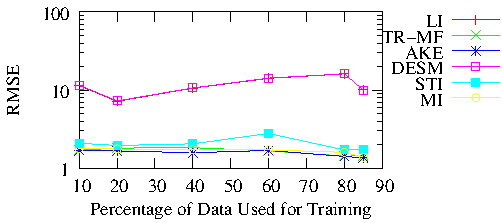
\includegraphics[width=0.45\textwidth]{table11_pspdftex.pdf}
%	\label{fig: 1}
%}
%\hspace{0in}
%\subfigure[subFig 2 caption]{
%	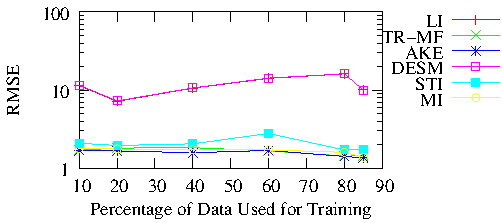
\includegraphics[width=0.45\textwidth]{table11_pspdftex.pdf}
%	\label{fig: 2}
%}
%
%\caption[nanana]{Global caption}
%\end{figure*}
